\documentclass{article}
\usepackage{pgfplots}
\pgfplotsset{compat=1.5}

\begin{document}
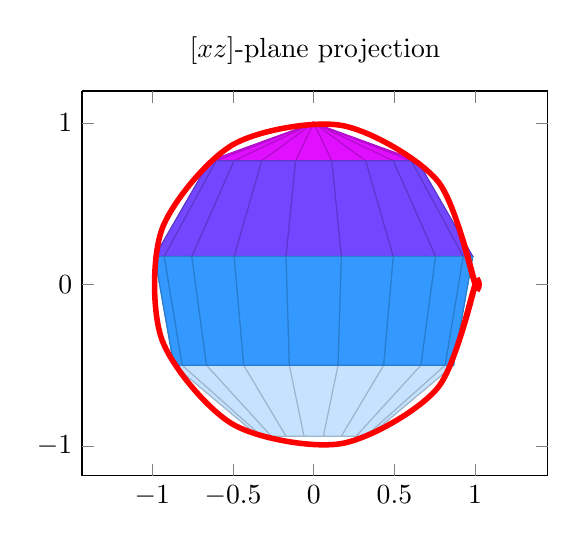
\begin{tikzpicture}
\begin{axis} [width=7.5cm, axis equal, view={0}{0}, title={$[xz]$-plane projection}]
\addplot3 [surf, z buffer=sort, samples=10, variable=\u, variable y=\v, domain=0:180, y domain=0:360,
           colormap/cool] ({cos(u)*sin(v)}, {sin(u)*sin(v)}, {cos(v)});
\addplot3 [domain=0:360, samples=10, smooth, variable=\t, line width=2pt, red] ({cos(t)}, {-2}, {sin(t)});
\end{axis}
\end{tikzpicture}
 
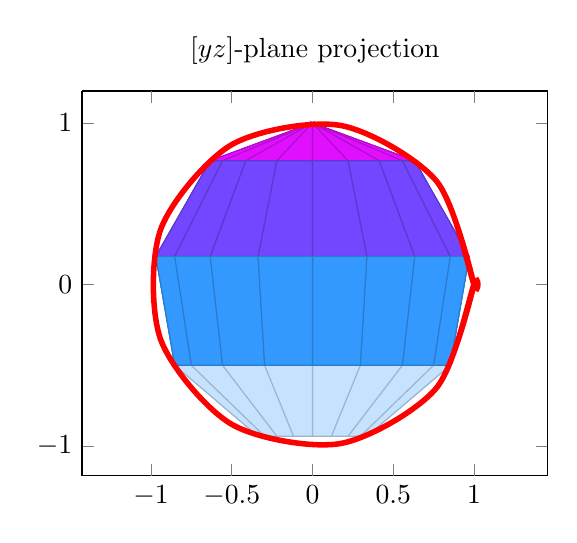
\begin{tikzpicture}
\begin{axis} [width=7.5cm, axis equal, view={90}{0}, title={$[yz]$-plane projection}]
\addplot3 [surf, z buffer=sort, samples=10, variable=\u, variable y=\v, domain=0:180, y domain=0:360,
           colormap/cool] ({cos(u)*sin(v)}, {sin(u)*sin(v)}, {cos(v)});
\addplot3 [domain=0:360, samples=10, smooth, variable=\t, line width=2pt, red] ({2}, {cos(t)}, {sin(t)});
\end{axis}
\end{tikzpicture}
 
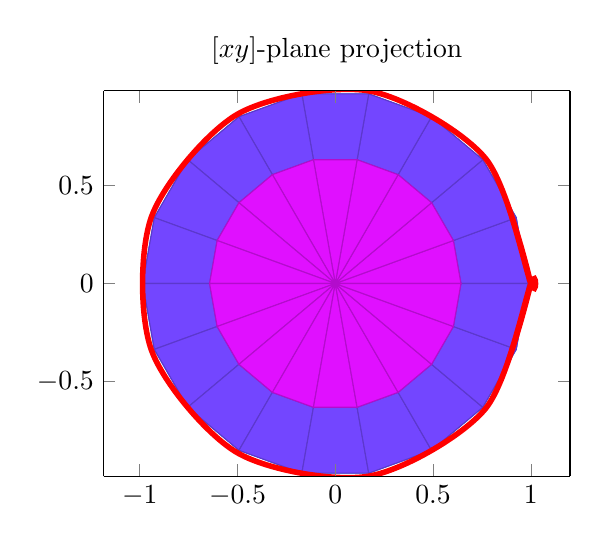
\begin{tikzpicture}
\begin{axis} [width=7.5cm, axis equal, view={0}{90}, title={$[xy]$-plane projection}]
\addplot3 [surf, z buffer=sort, samples=10, variable=\u, variable y=\v, domain=0:180, y domain=0:360,
           colormap/cool] ({cos(u)*sin(v)}, {sin(u)*sin(v)}, {cos(v)});
\addplot3 [domain=0:360, samples=10, smooth, variable=\t, line width=2pt, red] ({cos(t)}, {sin(t)}, {2});
\end{axis}
\end{tikzpicture}
\end{document}
